%% LyX 2.4.4 created this file.  For more info, see https://www.lyx.org/.
%% Do not edit unless you really know what you are doing.
\documentclass[english,t]{beamer}
\usepackage{mathptmx}
\usepackage[T1]{fontenc}
\usepackage[latin9]{inputenc}
\usepackage{amssymb}
\usepackage{cancel}

\makeatletter
%%%%%%%%%%%%%%%%%%%%%%%%%%%%%% Textclass specific LaTeX commands.
% this default might be overridden by plain title style
\newcommand\makebeamertitle{\frame{\maketitle}}%
% (ERT) argument for the TOC
\AtBeginDocument{%
  \let\origtableofcontents=\tableofcontents
  \def\tableofcontents{\@ifnextchar[{\origtableofcontents}{\gobbletableofcontents}}
  \def\gobbletableofcontents#1{\origtableofcontents}
}

%%%%%%%%%%%%%%%%%%%%%%%%%%%%%% User specified LaTeX commands.
\usetheme{Warsaw}
% or ...

\setbeamercovered{transparent}
% or whatever (possibly just delete it)
\setbeamercovered{invisible} %makes overlays invisible


%gets rid of navigation symbols
\setbeamertemplate{navigation symbols}{}

\usepackage{multicol}

\usepackage{tikz}
\usetikzlibrary{calc}
\usetikzlibrary{plotmarks}
\usepackage{pgfplots}
\pgfplotsset{compat=newest}

\usepackage{calc}
\usepackage[nomessages]{fp}

\usepackage{advdate}    % Advancing/saving dates
\usepackage{datetime}   % Dates formatting
\usepackage{datenumber} % Counters for dates

%\usepackage{pgfpages}
%\pgfpagesuselayout{4 on 1}[a4paper, landscape, border shrink=7mm]
%\pgfpageslogicalpageoptions{1}{border code=\pgfusepath{stroke}}
%\pgfpageslogicalpageoptions{2}{border code=\pgfusepath{stroke}}
%\pgfpageslogicalpageoptions{3}{border code=\pgfusepath{stroke}}
%\pgfpageslogicalpageoptions{4}{border code=\pgfusepath{stroke}}
%%%Don't forget to add 'handout'

\makeatother

\usepackage{babel}
\begin{document}
\newcommand{\xmax}{2000}
\newcommand{\xmin}{0}
\newcommand{\xstep}{0} %must be xmin+n
\newcommand{\ymax}{500}
\newcommand{\ymin}{0}
\newcommand{\ystep}{0} %must be ymin+n

\newcounter{countEx} \setcounter{countEx}{0}
\newcounter{countProb} \setcounter{countProb}{0}
\resetcounteronoverlays{countEx} \resetcounteronoverlays{countProb}

\newcommand{\ex}[3]{
	\addtocounter{countEx}{1}
	\only<#1-#2>{\begin{exampleblock} {Example \chNum.\secNum.\arabic{countEx}.} #3	\end{exampleblock}}
}

\newcommand{\prob}[4]{
	\addtocounter{countProb}{1}
	\only<#1-#2>{\begin{exampleblock} {Problem  \chNum.\secNum.\arabic{countProb}.\,#3} #4	\end{exampleblock}}
}

\newcommand{\yline}[4]{
	(#2 - #4)/(#1 - #3)*(x - #1) + #2
}

\beamerdefaultoverlayspecification{<+->}

%%%%Chapter and Section numbers%%%%%
\newcommand{\chNum}{2}
\newcommand{\secNum}{1}
\newcommand{\secTitle}{Systems of Linear Systems by the Echelon Method}

\title[Section \chNum.\secNum: \secTitle]{Section \chNum.\secNum: \secTitle}

\subtitle{Finite Mathematics~~MTH 132~~Spring 2014}

\author{Dr.\,James Ashe}

\titlegraphic{\includegraphics[height=1.5cm]{/home/jim/JamesAshe/JCSU/images/jcsu_bull}}

\institute{Johnson C. Smith University}

\date{{}}

\makebeamertitle 
\begin{frame}{Types of solutions for 2 equations with 2 unknowns }

\begin{block}<2->{}
Two or more linear equations involving the same set of variables
is called a \emph{system of linear equations}.
\end{block}
\begin{columns}


\column{3.5cm}
\begin{itemize}
\item []<3->$y=2x-8$
\item []<3->$y=-2x+4$
\item []<4->\textbf{Solve:} $2x-8=-2x+4$\emph{ }
\item []<5->\vspace{0cm}
%%%%%%%
\begin{tikzpicture} 
\begin{axis}[height=3.5cm, 
	width=3.5cm, axis lines=middle,
	minor x tick num={4},minor y tick num={4},
	grid=both,
	xmin=-10,
	xmax=10,
	ymin=-10,
	ymax=10,
	xlabel={$x$},ylabel={$y$}, 
	ticks=none,
	%xtick={0,50,...,250},%ytick={0,10,20,...,40},%axis line style={-latex},
every axis/.append style={font=\tiny},
	%restrict y to domain=-1:10,%no markers, 
	%every axis x label/.append style={anchor=north},%every axis y label/.append style={anchor=east}
	/pgf/number format/1000 sep={}
	]
	
	\only<5->{\addplot[thick,draw=red,domain=-10:10] {2*x-8} node[pos=.65,above] {$$};}
	\only<6->{\addplot[thick,draw=blue,domain=-10:10] {-2*x+4} node[pos=.65,above] {$$};}
  
	\only<7->{\addplot[draw=none,color=black,solid,very thick,mark=x,style={font=\footnotesize}] coordinates {(3,-2)};}
	
\end{axis}
\end{tikzpicture}
\end{itemize}

\column{3.5cm}
\begin{itemize}
\item []<3->$y=2x-8$
\item []<3->$y=2x+4$
\item []<8->\textbf{Solve:} $2x-8=2x+4$\emph{ }
\item []<9->\vspace{0cm}
%%%%%%%
\begin{tikzpicture} 
\begin{axis}[height=3.5cm, 
	width=3.5cm, axis lines=middle,
	minor x tick num={4},minor y tick num={4},
	grid=both,
	xmin=-10,
	xmax=10,
	ymin=-10,
	ymax=10,
	xlabel={$x$},ylabel={$y$}, 
	ticks=none,
	%xtick={0,50,...,250},%ytick={0,10,20,...,40},%axis line style={-latex},
every axis/.append style={font=\tiny},
	%restrict y to domain=-1:10,%no markers, 
	%every axis x label/.append style={anchor=north},%every axis y label/.append style={anchor=east}
	/pgf/number format/1000 sep={}
	]
	
	\only<10->{\addplot[thick,draw=red,domain=-10:10] {2*x-8} node[pos=.65,above] {$$};}
	\only<11->{\addplot[thick,draw=blue,domain=-10:10] {2*x+4} node[pos=.65,above] {$$};}
  
	%\only<12->{\addplot[draw=none,color=black,solid,very thick,mark=x,style={font=\footnotesize}] coordinates {(3,-2)};}
	
\end{axis}
\end{tikzpicture}
\end{itemize}

\column{3.5cm}
\begin{itemize}
\item []<3->$y=2x-8$
\item []<3->$y=2x-8$
\item []<12->\textbf{Solve:} $2x-8=2x-8$\emph{ }
\item []<13->\vspace{0cm}
%%%%%%%
\begin{tikzpicture} 
\begin{axis}[height=3.5cm, 
	width=3.5cm, axis lines=middle,
	minor x tick num={4},minor y tick num={4},
	grid=both,
	xmin=-10,
	xmax=10,
	ymin=-10,
	ymax=10,
	xlabel={$x$},ylabel={$y$}, 
	ticks=none,
	%xtick={0,50,...,250},%ytick={0,10,20,...,40},%axis line style={-latex},
every axis/.append style={font=\tiny},
	%restrict y to domain=-1:10,%no markers, 
	%every axis x label/.append style={anchor=north},%every axis y label/.append style={anchor=east}
	/pgf/number format/1000 sep={}
	]
	
	\only<13->{\addplot[thick,draw=red,domain=-10:10] {2*x-8} node[pos=.65,above] {$$};}
	\only<14->{\addplot[ very thick,draw=purple,domain=-10:10] {2*x-8} node[pos=.65,above] {$$};}
  
	%\only<7->{\addplot[draw=none,color=black,solid,very thick,mark=x,style={font=\footnotesize}] coordinates {(3,-2)};}
	
\end{axis}
\end{tikzpicture}
\end{itemize}
\end{columns}
\end{frame}

\begin{frame}{Solving Linear Systems by the Echelon Method}

\ex{1}{}{Use the echelon method to solve the system $y=2x-8$ and $y=-2x+4$}
\begin{columns}


\column{5.5cm}
\begin{itemize}
\item <3->[]$\begin{array}{rrrrr}
-2x & + & y & = & -8\\
2x & + & y & = & 4
\end{array}$
\end{itemize}

\column{5.5cm}

\vspace{-.525cm}
\begin{block}<2->{step 1}
Write the system aligning the $x$'s, $y$'s, and constants along
columns
\end{block}

\begin{block}<4->{step 2}
Eliminate one of the variables, and solve.
\end{block}

\begin{block}<5->{step 3}
Substitute the solution from \emph{step 2 }to find the remaining
variable.
\end{block}
\end{columns}
\end{frame}

\begin{frame}{}

\begin{columns}


\column{5.5cm}

\column{5.5cm}

\ex{1}{}{Solve the system $\begin{array}{rrrrr} -3x & + & y & = & 4\\ 2x & - & 2y & = & -4 \end{array}$}
\end{columns}
\end{frame}

\begin{frame}{}

\begin{columns}


\column{5.5cm}

\ex{1}{}{Solve the system $\begin{array}{rrrrr} 9x & - & 5y & = & 1\\ -18x & + & 10y & = & 1 \end{array}$}

\column{5.5cm}

\end{columns}
\end{frame}

\begin{frame}{}

\ex{1}{}{A shop sells skirts for \$45 and pants for \$35. Its entire stock is worth \$51,750. During their big sale, half the skirts and two-thirds of the pants were sold for \$30,600. How many skirts and pants are left in stock?}
\end{frame}

\begin{frame}{}

\begin{columns}


\column{5.5cm}

\ex{1}{}{Solve the system $\begin{array}{rrrrr} 45p & + & 35s & = & 51,750\\ \frac{2}{3}45p & + & \frac{1}{2}35s & = & 30,600 \end{array}$}

\column{5.5cm}

\end{columns}
\end{frame}

\begin{frame}{}

\prob{1}{}{Solve the system}{\hfill $\begin{array}{rrrrr} 6x & - & 2y & = & -4\\ 3x & + & 4y & = & 8 \end{array}$ \hfill}
\begin{itemize}
\item <2->[]Answer: $(0,2)$
\end{itemize}
\end{frame}

\end{document}
